%%%----------------------------------------------------------
\chapter{Affine Point Cloud Matching}
%%%----------------------------------------------------------

In this assignment the task was to find the affine transformation between two point sets. At first a thought experiment should be done about how long it would take if to match the two point sets by brute force and if that would be a reasonable approach. In the second task the affine transformation between two point sets is given and it needs to be applied to check if the transformation is done right. The third task was about finding the affine transformation between two point sets with the help of a method called triangulation.

\section{Matching point sets by brute force or RANSAC}

As described in the last assignment (\autoref{chap:ass01}) the RANSAC method can be an efficient way to find a solution. But can it also be used to find the correspondence between two point sets? How long would it take to find the affine transformation between two point sets by randomly or systematically picking three points in both point clouds? The following thought experiment discusses these questions:

Let's assume that we have two images with $m$ points and we are picking systematically $n$ points in each point cloud there would be 
 \begin{equation}
 	\frac{m!}{(m-n)!}
\end{equation}
possible combinations. To find the best possible solution we need do same with the points in the second image which results in the following equation provided the number of points in both point clouds is the same:
\begin{equation}
	\left(\frac{m!}{(m-n)!}\right)^2
\end{equation}
As we can see the growth is exponential and the number of possibilities would get really high really fast with an increasing number of points $m$.

\subsection{Research Question 1}

\begin{itshape}
	If your computer could perform 1 million such tests per second, how long would it take to examine all possible 3-point matches, if m = 10, 50, 1000?	
\end{itshape}

\begin{align}
	\frac{\left(\frac{10!}{(10-3)!}\right)^2}{1000000}& \approx 0.52s\\
	\frac{\left(\frac{50!}{(50-3)!}\right)^2}{1000000}& \approx 3.84h\\
	\frac{\left(\frac{1000!}{(1000-3)!}\right)^2}{1000000}& \approx 31520 years
	\label{timeForTest1000}
\end{align}

While 0.52 seconds for 10 points does not sound that bad, 3.84 hours for 50 points sounds already unusable and 31520 years by far exceeds any time limit for a human being. Considering that point clouds often exceed 1000 points by quite a bit nowadays proves that using a brute-force approach to find the correspondence between two point clouds is not an option.

\subsection{Research Question 2}

\begin{itshape}
	Why would the RANSAC approach (as used successfully in Assignment 1) not be of much help in this case?
\end{itshape}

Since the points also need to be chosen in the correct order in both point sets the chance to randomly select the correct 3 points in both sets is very low. The number of possibilities are way to high to use the RANSAC approach.

\section{Implement and test the affine transformation}

The true transformation between point set $X$ and $X'$ is given:
\begin{equation}
\label{eq:transMatrix}
	A = 
	\begin{pmatrix}
		a_{00} & a_{01} & a_{02} \\
		a_{10} & a_{11} & a_{12} \\
	\end{pmatrix} 
	=
	\begin{pmatrix}
		0.013 & 1.088 & 18.688 \\
		-1.000 & - 0.050 & 127.500\\
	\end{pmatrix}
\end{equation}

An affine transformation can be expressed as a matrix-vector multiplication:
\begin{equation}
	\begin{pmatrix}
		x' \\
		y' \\
		1
	\end{pmatrix}
	= 
	\begin{pmatrix}
		a_{00} & a_{01} & a_{02} \\
		a_{10} & a_{11} & a_{12} \\
		0 & 0 & 1 \\
	\end{pmatrix} 
	\cdot
	\begin{pmatrix}
		x \\
		y \\
		1
	\end{pmatrix}
\end{equation}

The given transformation matrix was applied to each point of the first point set and then the closest point in the second point set was calculated which is considered the corresponding point. The residual error is the sum of the distance between the calculated position and the position of their respective corresponding point over all points. 

\subsection{Result}

In Figure \ref{fig:TestTransInput} both point sets are shown in one image. Figure \ref{fig:TestTransResult} shows the result after applying the given transformation matrix to the red point set. The residual error resulted in 1.0 which was caused by the rounding error over time. 

\begin{figure}
	\centering
	\begin{minipage}[t]{0.49\linewidth}
		\centering
		\frame{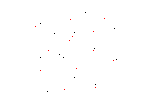
\includegraphics[width=.95\linewidth]{images/ass02TestTransInput}}
		\caption{Both point sets.}
		\label{fig:TestTransInput}
	\end{minipage}
	\hfill
	\begin{minipage}[t]{0.49\linewidth}
		\centering
		\frame{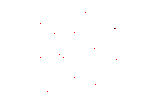
\includegraphics[width=.95\linewidth]{images/ass02TestTransResult}}
		\caption{After applying the given transformation to the red point set.}
		\label{fig:TestTransResult}
	\end{minipage}
\end{figure}

\section{Structuring point sets by triangulation}

As stated in the first Task using either brute-force or the RANSAC algorithm to find point correspondence is not a valid solution for bigger point sets. In this task the problem should be solved by applying the \textit{Delaunay triangulation}\cite{Delaunay2020}. This approach always connects 3 points of a point set to triangles. Figure \ref{fig:DelunayTri} shows the two triangulated example point clouds.

\begin{figure}
	\centering
	\begin{minipage}[t]{0.49\linewidth}
		\centering
		\frame{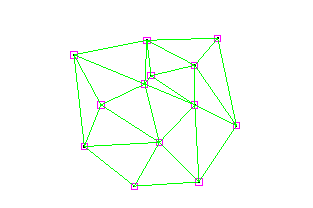
\includegraphics[width=.95\linewidth]{images/ass02TriFirst.pdf}}
	\end{minipage}
	\hfill
	\begin{minipage}[t]{0.49\linewidth}
		\centering
		\frame{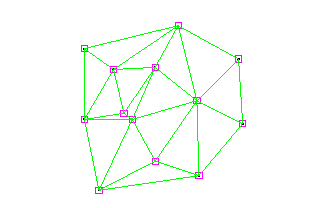
\includegraphics[width=.95\linewidth]{images/ass02TriSec.pdf}}
	\end{minipage}
	\caption{Delunay triangulation.}
	\label{fig:DelunayTri}
\end{figure}


\subsection{Algorithm}

\begin{enumerate}
	\item Calculate the Delaunay triangulation for both point sets.
	\item Iterate through all triangles  from $X$ and $X'$ and for each pair perform the following steps:
		\begin{itemize}
			\item Find the affine transformation $A$ between them.
			\item Apply $A$ to all points in $X$ and calculate the error of the projected points to the closest points in $X'$.
			\item Check for permutation within the triangles.
			\item Memorize the best-fit with the smallest error.
		\end{itemize}
	\item Find the best least-squares fit for the resulting point match.
\end{enumerate}

\subsection{Calculate the Delaunay Triangulation}

A library for the triangulation was provided which returns a set of triangles for each point set.

\subsection{Iterate through all triangles}

For each triangle of the the first set we iterate over the triangles in the second set. Between each triangle pair the corresponding point pairs ($x_0, x'_0$), ($x_1, x'_1$), ($x_2, x'_2$) are formed. The next step was to find the 6 needed parameters for the affine transformation. To find these parameter at least 6 equations were needed to find these 6 unknowns. With the help of the 3 point pairs a linear equation system was created:
\begin{align*}
	x'_0& = a_{00}\cdot x_0 + a_{01} \cdot y_0 + a_{02} \\
	y'_0& = a_{10}\cdot x_0 + a_{11} \cdot y_0 + a_{12} \\
	x'_1& = a_{00}\cdot x_1 + a_{01} \cdot y_1 + a_{02} \\
	y'_1& = a_{10}\cdot x_1 + a_{11} \cdot y_1 + a_{12} \\
	x'_2& = a_{00}\cdot x_2 + a_{01} \cdot y_2 + a_{02} \\
	y'_2& = a_{10}\cdot x_2 + a_{11} \cdot y_2 + a_{12} \\
\end{align*}

To be able to solve this system with the provided linear equation system solver the system needed to be rearranged into this general form:
\begin{equation}
	M \cdot a = b
\end{equation}

Which resulted in following matrix-vector form:
\begin{equation}
	\begin{pmatrix}
		x_0 & y_0 & 1 & 0 & 0 & 0 \\
		0 & 0 & 0 & x_0 & y_0 & 1 \\
		x_1 & y_1 & 1 & 0 & 0 & 0 \\
		0 & 0 & 0 & x_1 & y_1 & 1 \\
		x_2 & y_2 & 1 & 0 & 0 & 0 \\
		0 & 0 & 0 & x_2 & y_2 & 1 \\
	\end{pmatrix} 
	\cdot
	\begin{pmatrix}
		a_{00} \\
		a_{01} \\
		a_{02} \\
		a_{10} \\
		a_{11} \\
		a_{12} \\
	\end{pmatrix}
	=
	\begin{pmatrix}
		x'_0 \\
		y'_0 \\
		x'_1 \\
		y'_1 \\
		x'_2 \\
		y'_2
	\end{pmatrix}
\end{equation}

After solving that equation all parameters for the affine transformation were calculated ($a_{00}, a_{01} \ldots a_{12}$). With these parameters the transformation matrix $A$ was created.

\subsection{Find the best least-squares fit.}
Once the Transformation $A$ was known it was applied to all points in the point set $X$. The Euclidean squared distances were calculated between each point and it's assumed corresponding point and summed up. The resulting error was compared to the error of the last best-fitting transformation. The transformation with the smallest error was remembered. After iterating through both triangle sets the transformation resulting in the smallest error was known.

\subsection{Result}
The squared error of the best fit for the test images was 8.64 and the calculated transformation matrix $A$ was:

\begin{equation}
	A = 
	\begin{pmatrix}
		0.019 & 1.096 & 17.827 \\
		-0.981 & -0.046 & 126.541 \\
	\end{pmatrix} 
\end{equation}

Which was pretty close to the originally provided matrix \ref{eq:transMatrix}. The comparison between the provided result and the transformed points can also be seen in Figure \ref{fig:TriResult}.

\begin{figure}
	\centering
	\frame{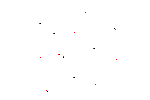
\includegraphics[width=.60\linewidth]{images/ass02TriResult}}
	\caption{Black dots: The real result points. Red dots: the transformed points.}
	\label{fig:TriResult}
\end{figure}

\subsection{Research Question}
\begin{itshape}
	When using the Delaunay triangulation for structuring corresponding point sets we implicitly assumed that the triangulation is insensitive to affine transformations in 2D. Is this really true? What would be needed to validate this assumption? Make a quick internet search and document your findings.	
\end{itshape}

In theory the Delaunay triangulation is invariant for translation, rotation and uniform scaling. However, triangulation of a point set is not stable and very sensitive to noise which can deliver different results.







